\section{Grid vs Sample Based Planning}
\label{sec:grid_vs_sample_based_planning}

So far we have limited our analysis and comparisons between the grid-based and the sample-based algorithms to a fixed set of predefined scenarios.
In this section, we further investigate the performance and capabilities of the two classes of algorithms by running specific tests that are designed to highlight their strengths and weaknesses.

Thanks to the flexibility provided by the rewiring mechanism of RRT*, in this section we are going to compare the performance of the A* against the RRT* algorithm.


\subsection{Path Asymptotic Optimality}
\label{subsec:path_optimality}

As already largely discussed in the previous sections, the main difference between grid-based and sample-based algorithms is that the former are guaranteed to find the optimal path, while the latter are not.
Formally, this statement has also been expressed in the literature by \cite{rrt_optimality}, which has proven that RRT can produce arbitrarily-bad paths with non-negligible probability.

We can also observe this behavior in our implementation of the RRT* algorithm.
Figure \ref{fig:04_path_optimality} shows the path generated by RRT* on the left and the path generated by A* on the right.

\begin{figure}[H]
    \centering
    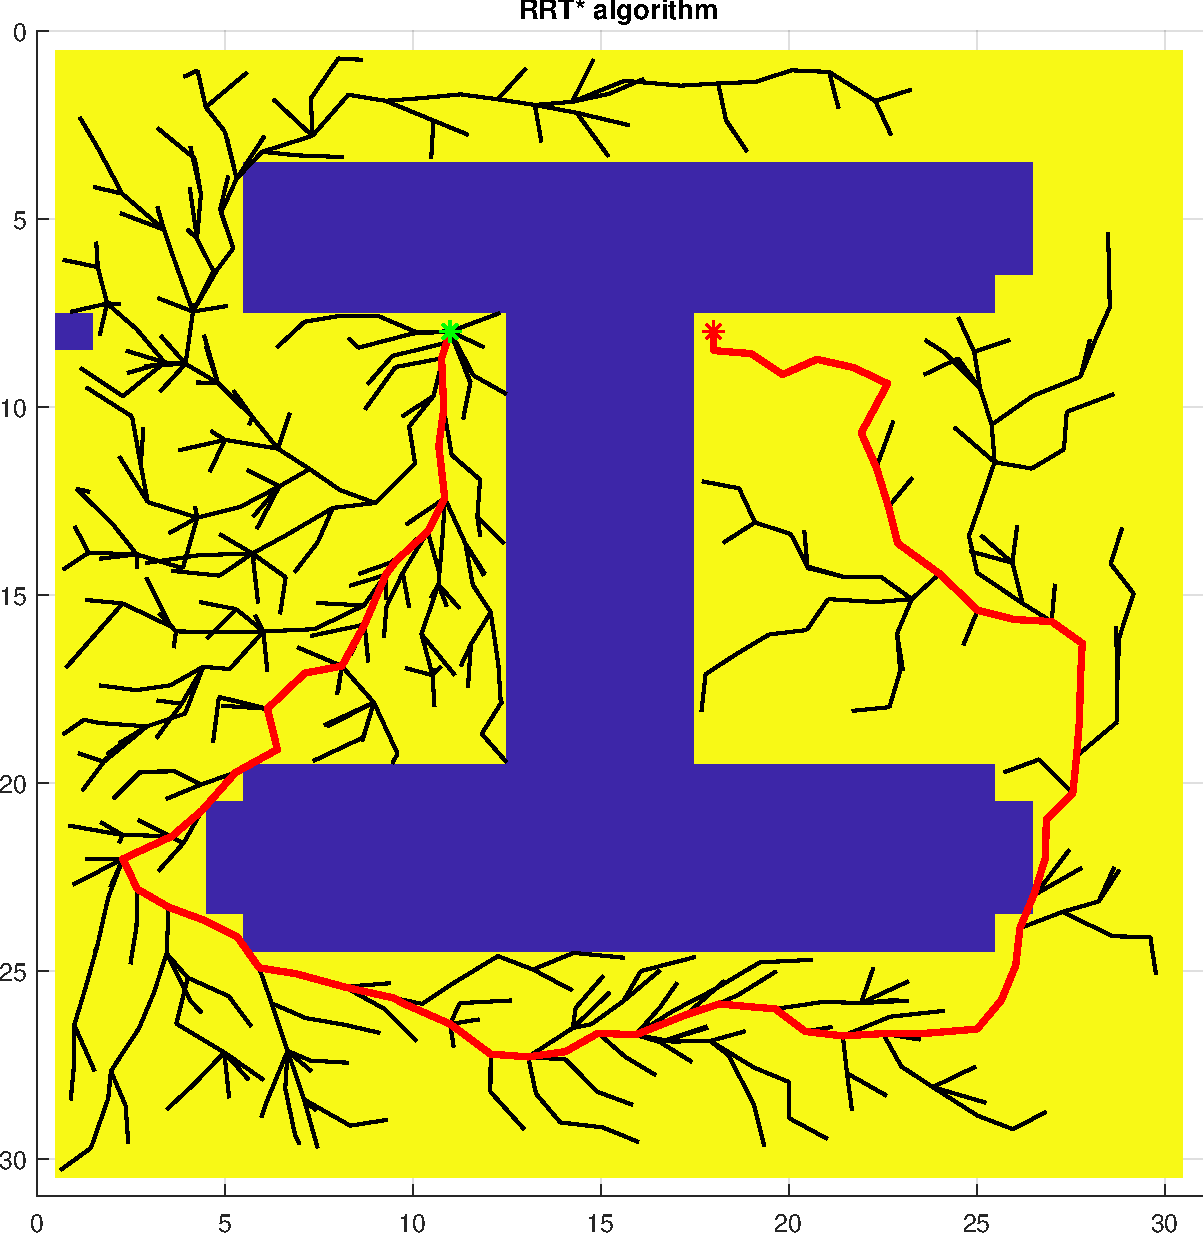
\includegraphics[width=0.48\textwidth]{./img/MATLAB/optimality/04_rrt_star_path_optimality.pdf}
    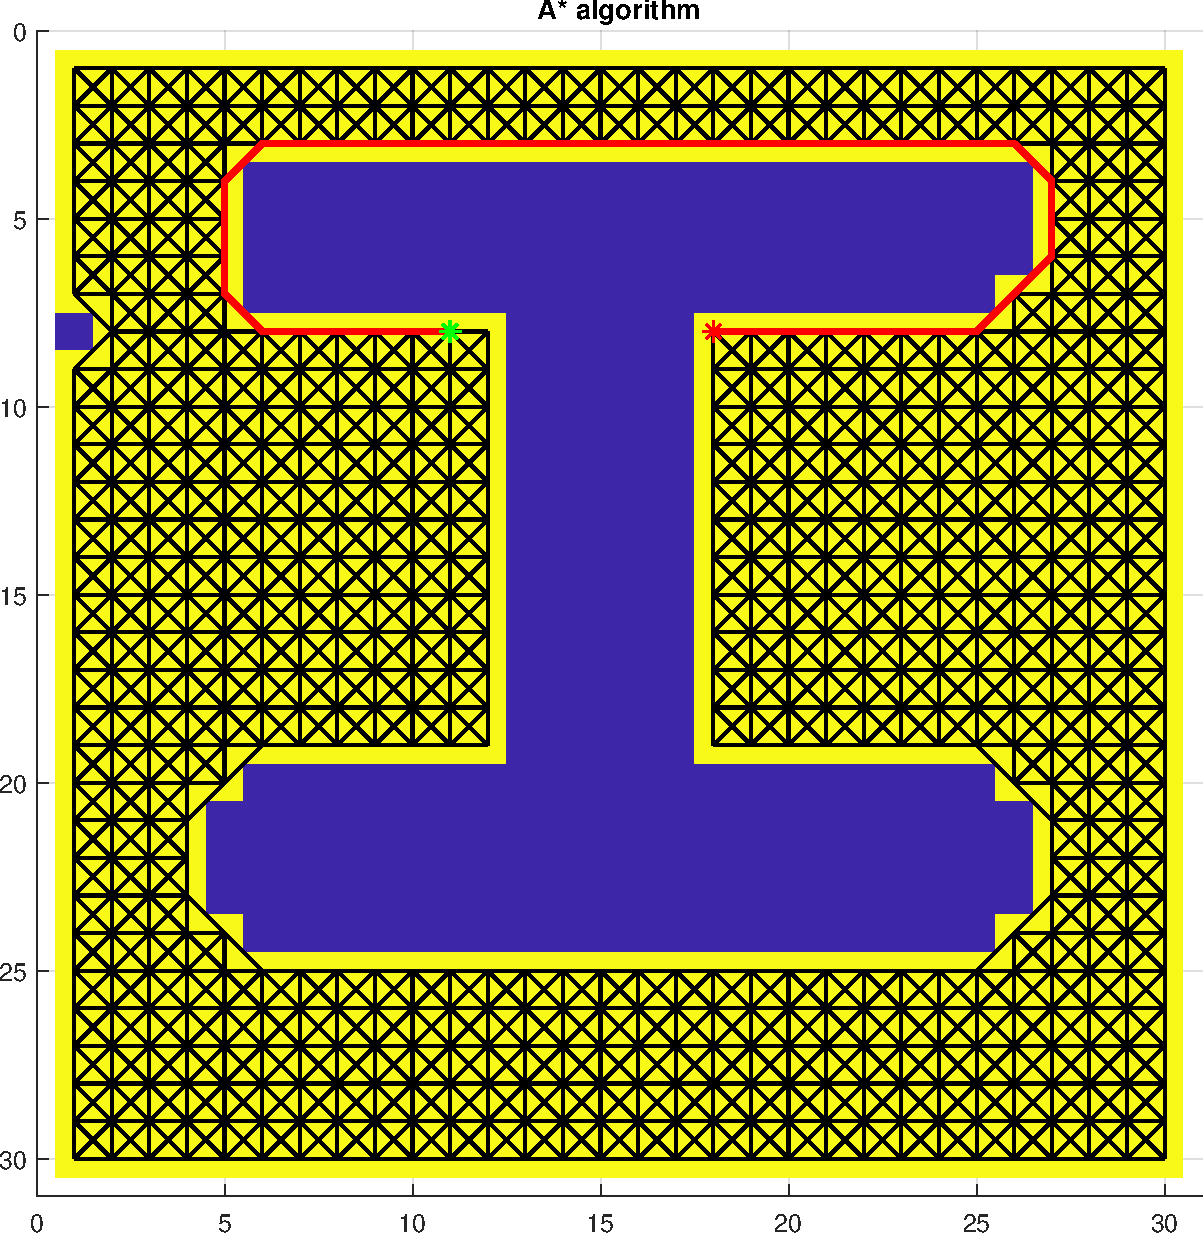
\includegraphics[width=0.48\textwidth]{./img/MATLAB/optimality/04_a_star_path_optimality.pdf}
    \caption{Path generated by RRT* (left) and A* (right) on the same scenario.}
    \label{fig:04_path_optimality}
\end{figure}

The path generated by RRT* is clearly suboptimal, choosing a much longer path only because fewer obstacles are present in that area and so higher chances of connectivity for the randomly generated nodes are present.

A similar case is shown in Figure \ref{fig:circle_path_optimality}.

\begin{figure}[H]
    \centering
    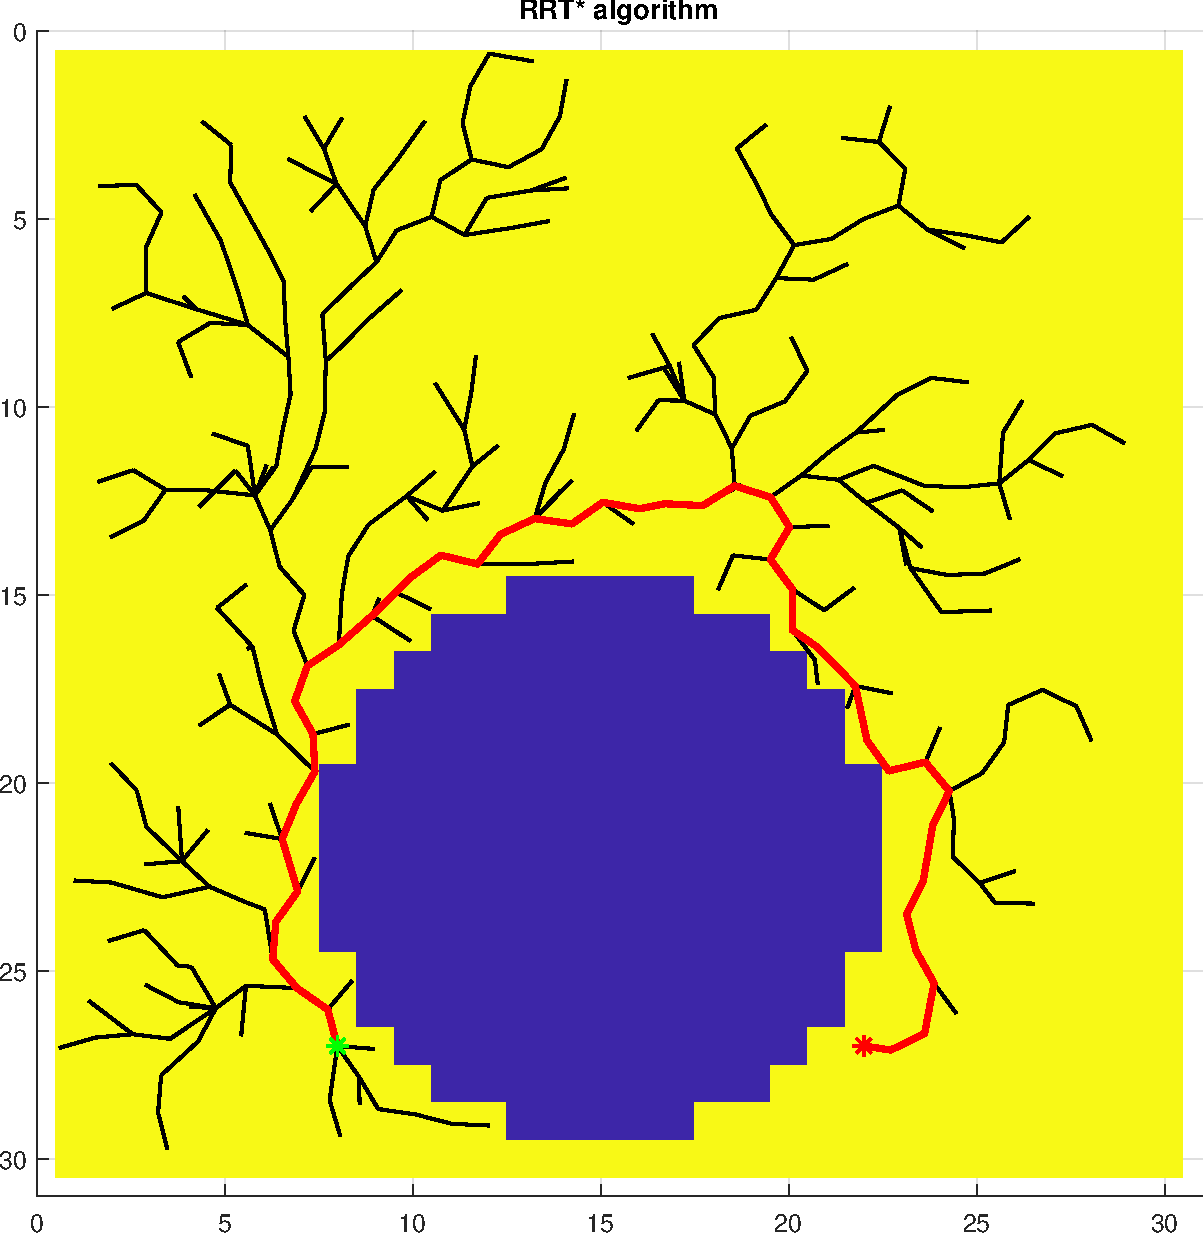
\includegraphics[width=0.48\textwidth]{./img/MATLAB/optimality/circle_rrt_star_path_optimality.pdf}
    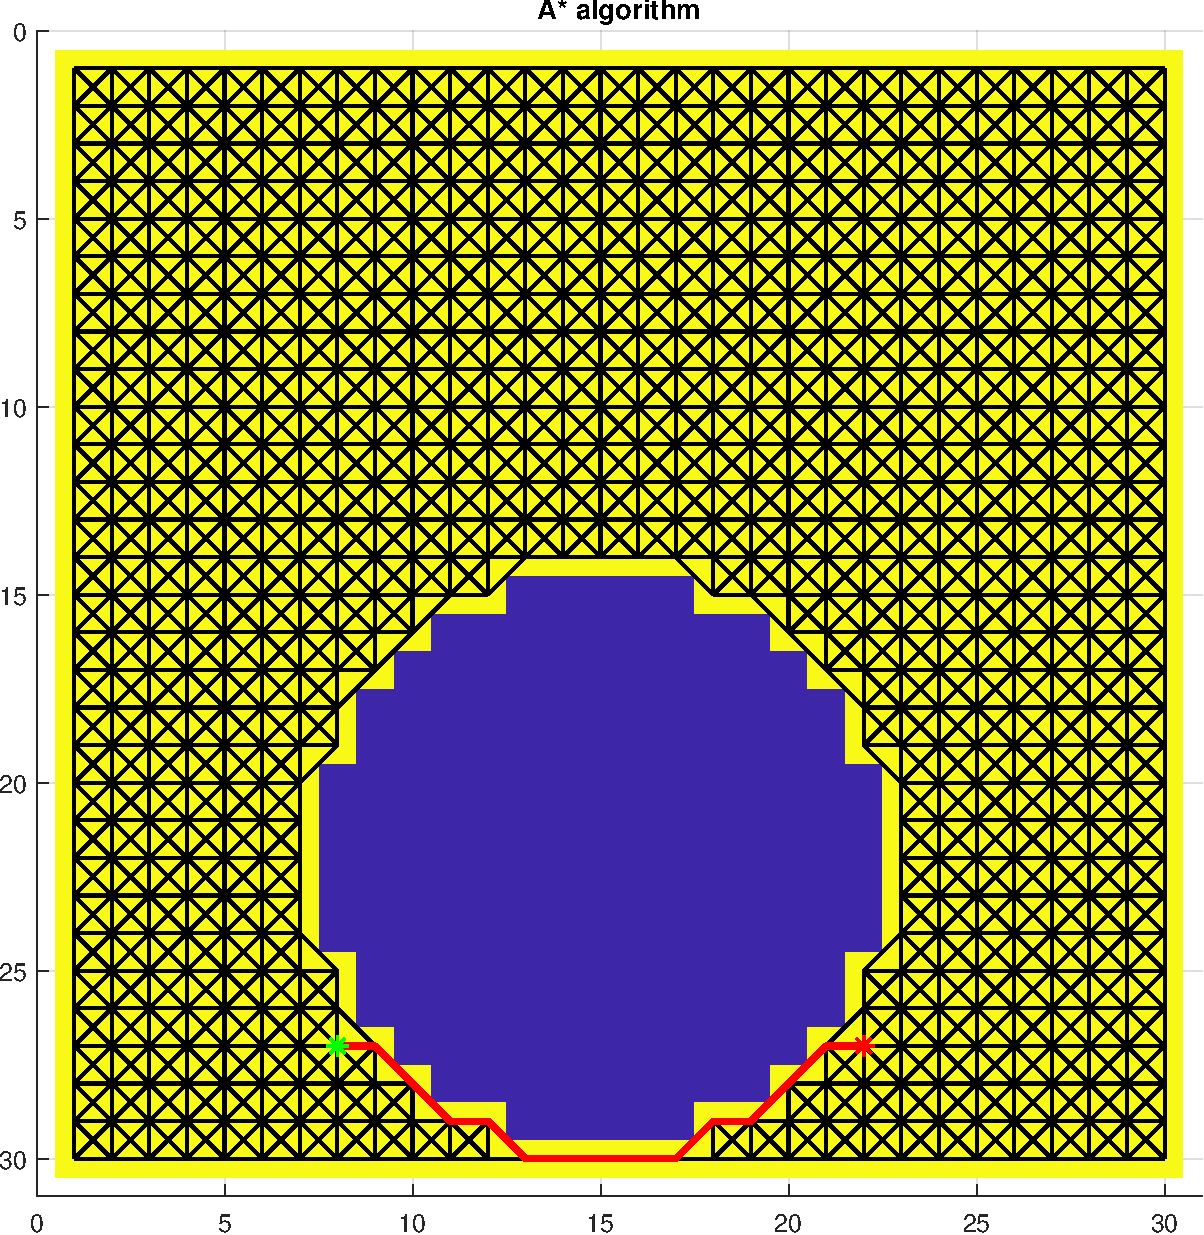
\includegraphics[width=0.48\textwidth]{./img/MATLAB/optimality/circle_a_star_path_optimality.pdf}
    \caption{Path generated by RRT* (left) and A* (right) on the same scenario.}
    \label{fig:circle_path_optimality}
\end{figure}

However, the RRT* algorithm is asymptotically optimal, meaning that the higher the number of nodes that the algorithm place, the more optimal the path becomes.
This is a very important property, as it allows trading off between the time spent in finding a solution and the quality of the solution itself.

By removing the interruption of the algorithm after the first solution is found, we can observe how the path generated by RRT* becomes more and more optimal as the number of iterations increases.
Figure \ref{fig:04_rrt_star_path_optimality_asymptotic} shows the path generated by RRT* after 1000 iterations on two different scenarios.
One can appreciate how, despite the number of iterations, in the case of the circle the path is still suboptimal.

\begin{figure}[H]
    \centering
    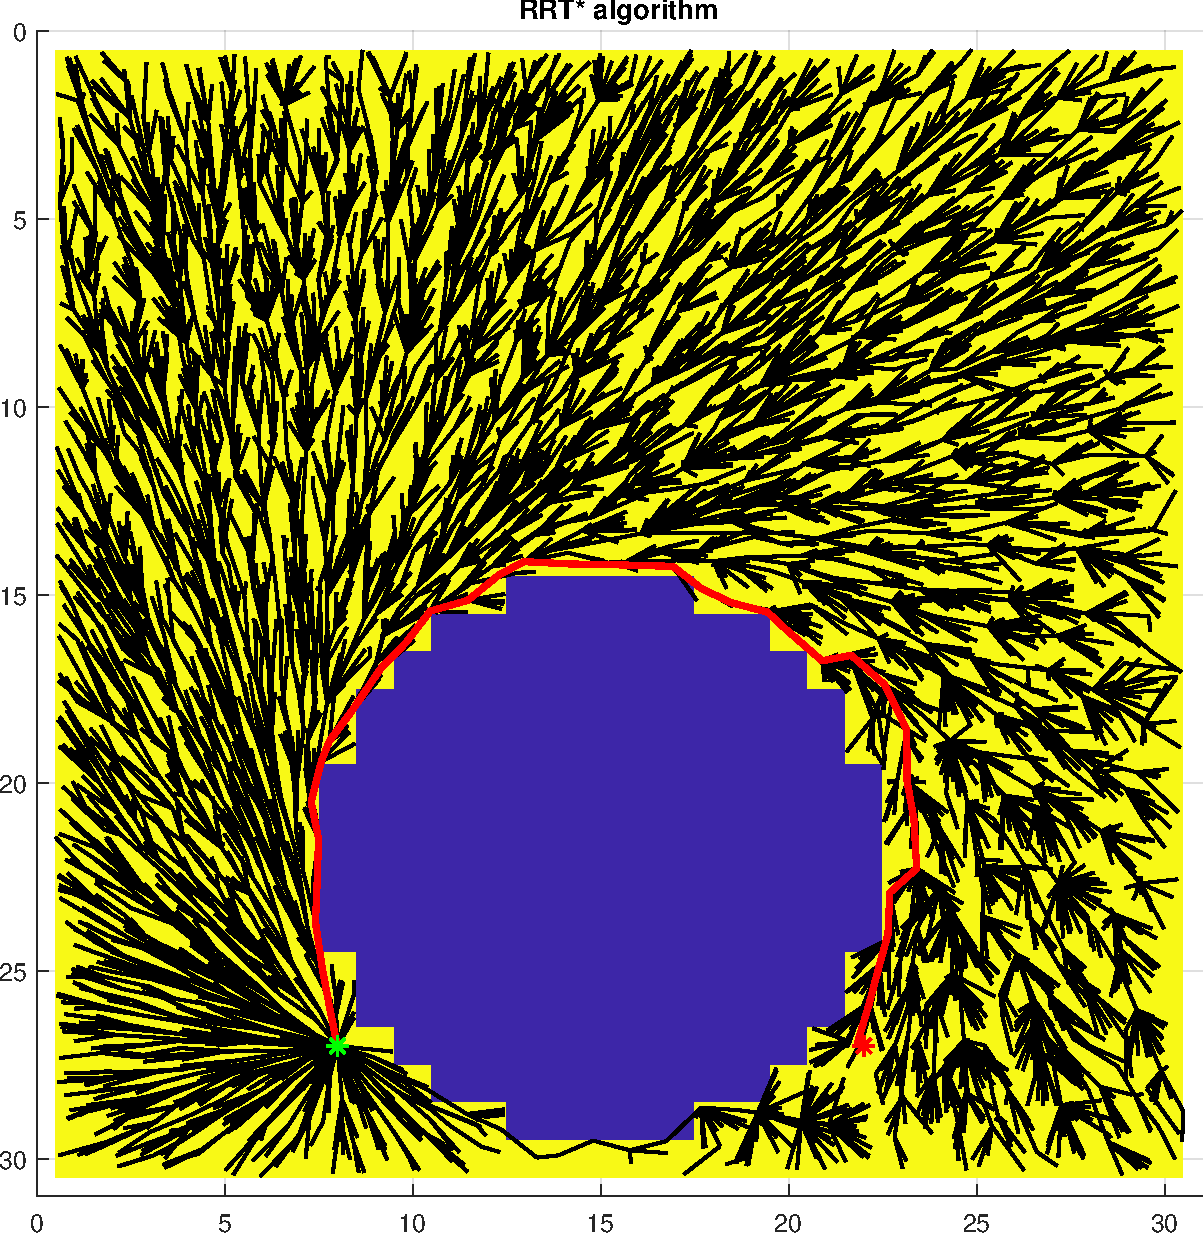
\includegraphics[width=0.48\textwidth]{./img/MATLAB/optimality/circle_rrt_star_path_optimality_10000.pdf}
    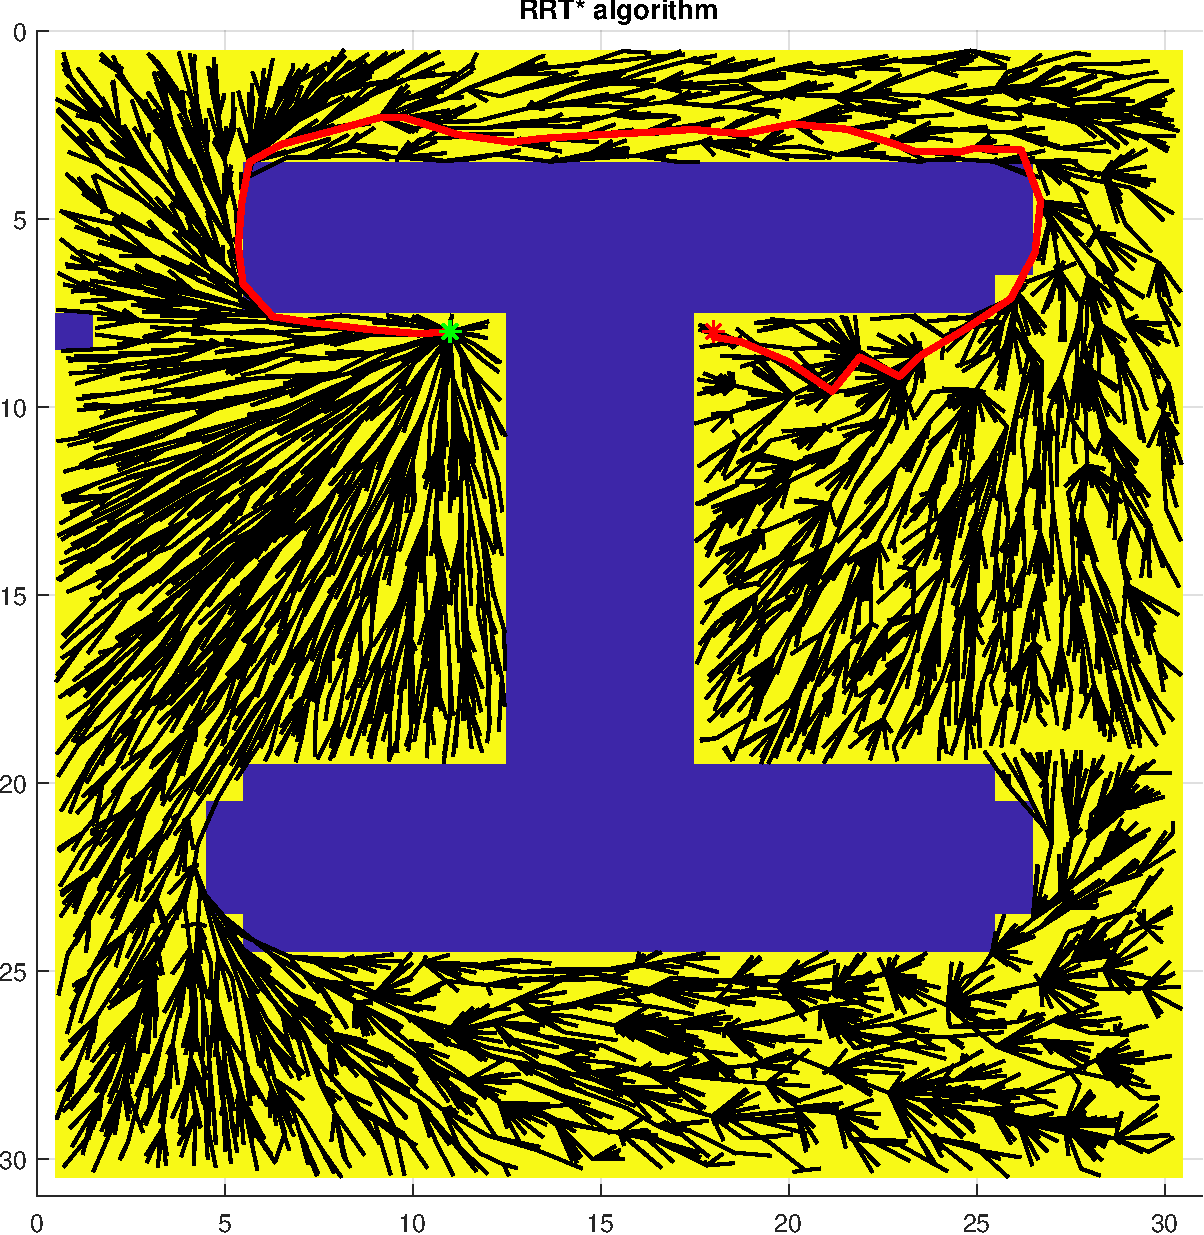
\includegraphics[width=0.48\textwidth]{./img/MATLAB/optimality/04_rrt_star_path_optimality_10000.pdf}
    \caption{Asymptotic optimality of RRT* algorithm. Both the images refer to 10000 iterations of the algorithm.}
    \label{fig:04_rrt_star_path_optimality_asymptotic}
\end{figure}

In Table \ref{tab:04_rrt_star_path_optimality_asymptotic} are reported the path length and the time taken by RRT* algorithm as a function of the number of iterations performed.
Results are relative to the right-hand side scenario of Figure \ref{fig:04_rrt_star_path_optimality_asymptotic}.

\begin{table}[H]
    \centering
    \begin{tabular}{|c|c|c|}
        \hline
        \textbf{Iterations} & \textbf{Path length (m)} & \textbf{Elapsed time (ms)} \\
        \hline
        1000                & 68                       & 324                        \\
        5000                & 60                       & 12775                      \\
        10000               & 44                       & 69069                      \\
        \hline
    \end{tabular}
    \caption{Path length and time taken by RRT* algorithm after different number of iterations.}
    \label{tab:04_rrt_star_path_optimality_asymptotic}
\end{table}

As expected, the path length decreases as the number of iterations increases, but the time taken by the algorithm increases significantly.
Thinking about deploying the algorithm on a real robot which needs the planner component to run in real-time or nearly real-time, we clearly understand that the number of iterations must be limited, and asymptotic optimality is not a property that can be exploited in practice.



\subsection{Multidimensional Workspace}
\label{subsec:multidimensional_workspace}

In this section we analyze the performance of the two algorithms on a 3D scenario, adding a third dimension to the problem.
The scenario is composed of a 3D grid of obstacles, which are randomly generated in the space.
Figure \ref{fig:3D_obstacles} shows a 3D view of the scenario and a stack of slicing along the Z axis.

\begin{figure}[H]
    \centering
    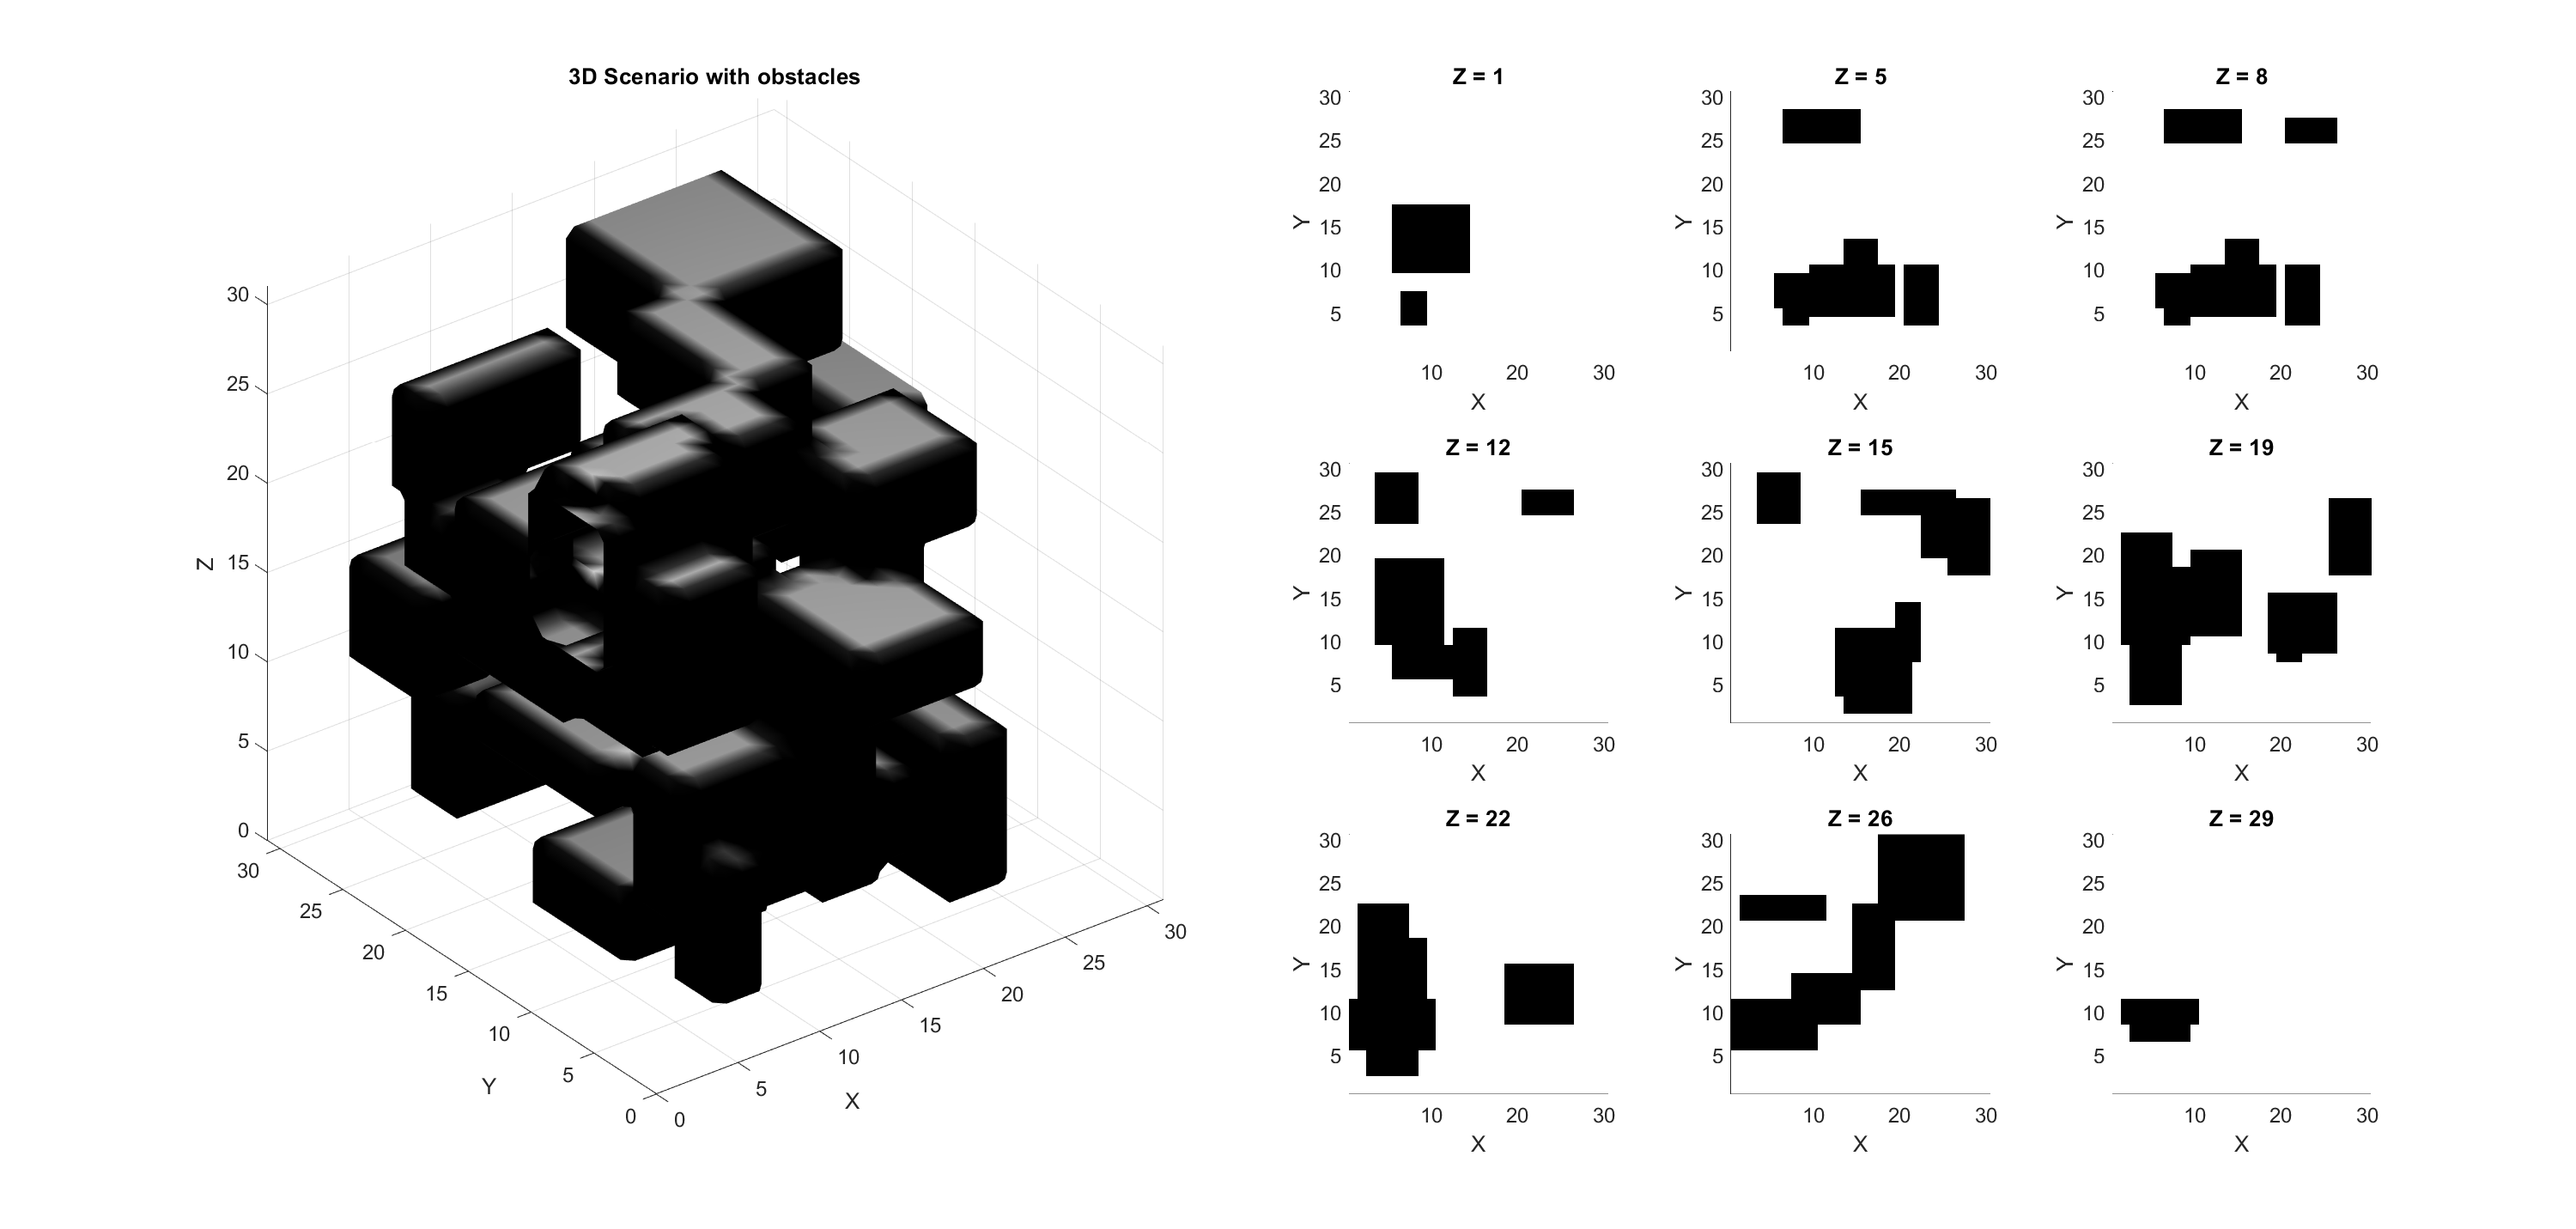
\includegraphics[width=1.0\textwidth]{./img/MATLAB/multidim/3D_obstacles.pdf}
    \caption{3D grid of obstacles used as a scenario for the tests.}
    \label{fig:3D_obstacles}
\end{figure}

With zero-to-little modifications to the algorithms, we run both the grid-based and the sample-based algorithms on the same 3D scenario.
Thanks to the increased dimensions of the problem, we clearly observe the huge difference in performance between the two class of algorithms.
Table \ref{tab:3D_grid_vs_sample_based} summarizes the results of the tests, while Figure \ref{fig:3D_grid_vs_sample_based} shows the paths generated by A*, RRT and RRT* algorithms.

\begin{table}[H]
    \centering
    \begin{tabular}{|c|c|c|c|}
        \hline
        \textbf{Algorithm} & \textbf{Elapsed time (ms)} & \textbf{Tree dimension} & \textbf{Path length (m)} \\
        \hline
        A*                 & 2435229 ($\sim$40[min])    & 20803                   & 87                       \\
        RRT                & 55                         & 191                     & 69                       \\
        RRT*               & 273                        & 397                     & 69                       \\
        \hline
    \end{tabular}
    \caption{Path length and time taken by each algorithm on the same 3D scenario.}
    \label{tab:3D_grid_vs_sample_based}
\end{table}

One can notice that the path generated by A* is longer than the one generated by RRT and RRT*.
This can be explained by the fact that the graph used to represent the workspace has been generated without allowing diagonal connections.
This means that, considering a 3D unitary volume of the grid, for the A* to go from one corner to the opposite one, it needs to go through all the 3 cells edges, while instead the RRT and RRT* algorithms are able to directly connect the two corners, without going through all the intermediate cells.
Thanks to this observation, a simple math shows that on average, if the diagonal connection were allowed, the path length would have been reduced by a factor of $\sqrt{3}$.
This means that the path length generated by A* would have been around $\frac{87}{\sqrt{3}} \approx 50$ m, which is lower than the path length generated by RRT and RRT*, indeed proving once again the concept of optimality of the grid-based algorithms.


\begin{figure}[H]
    \centering
    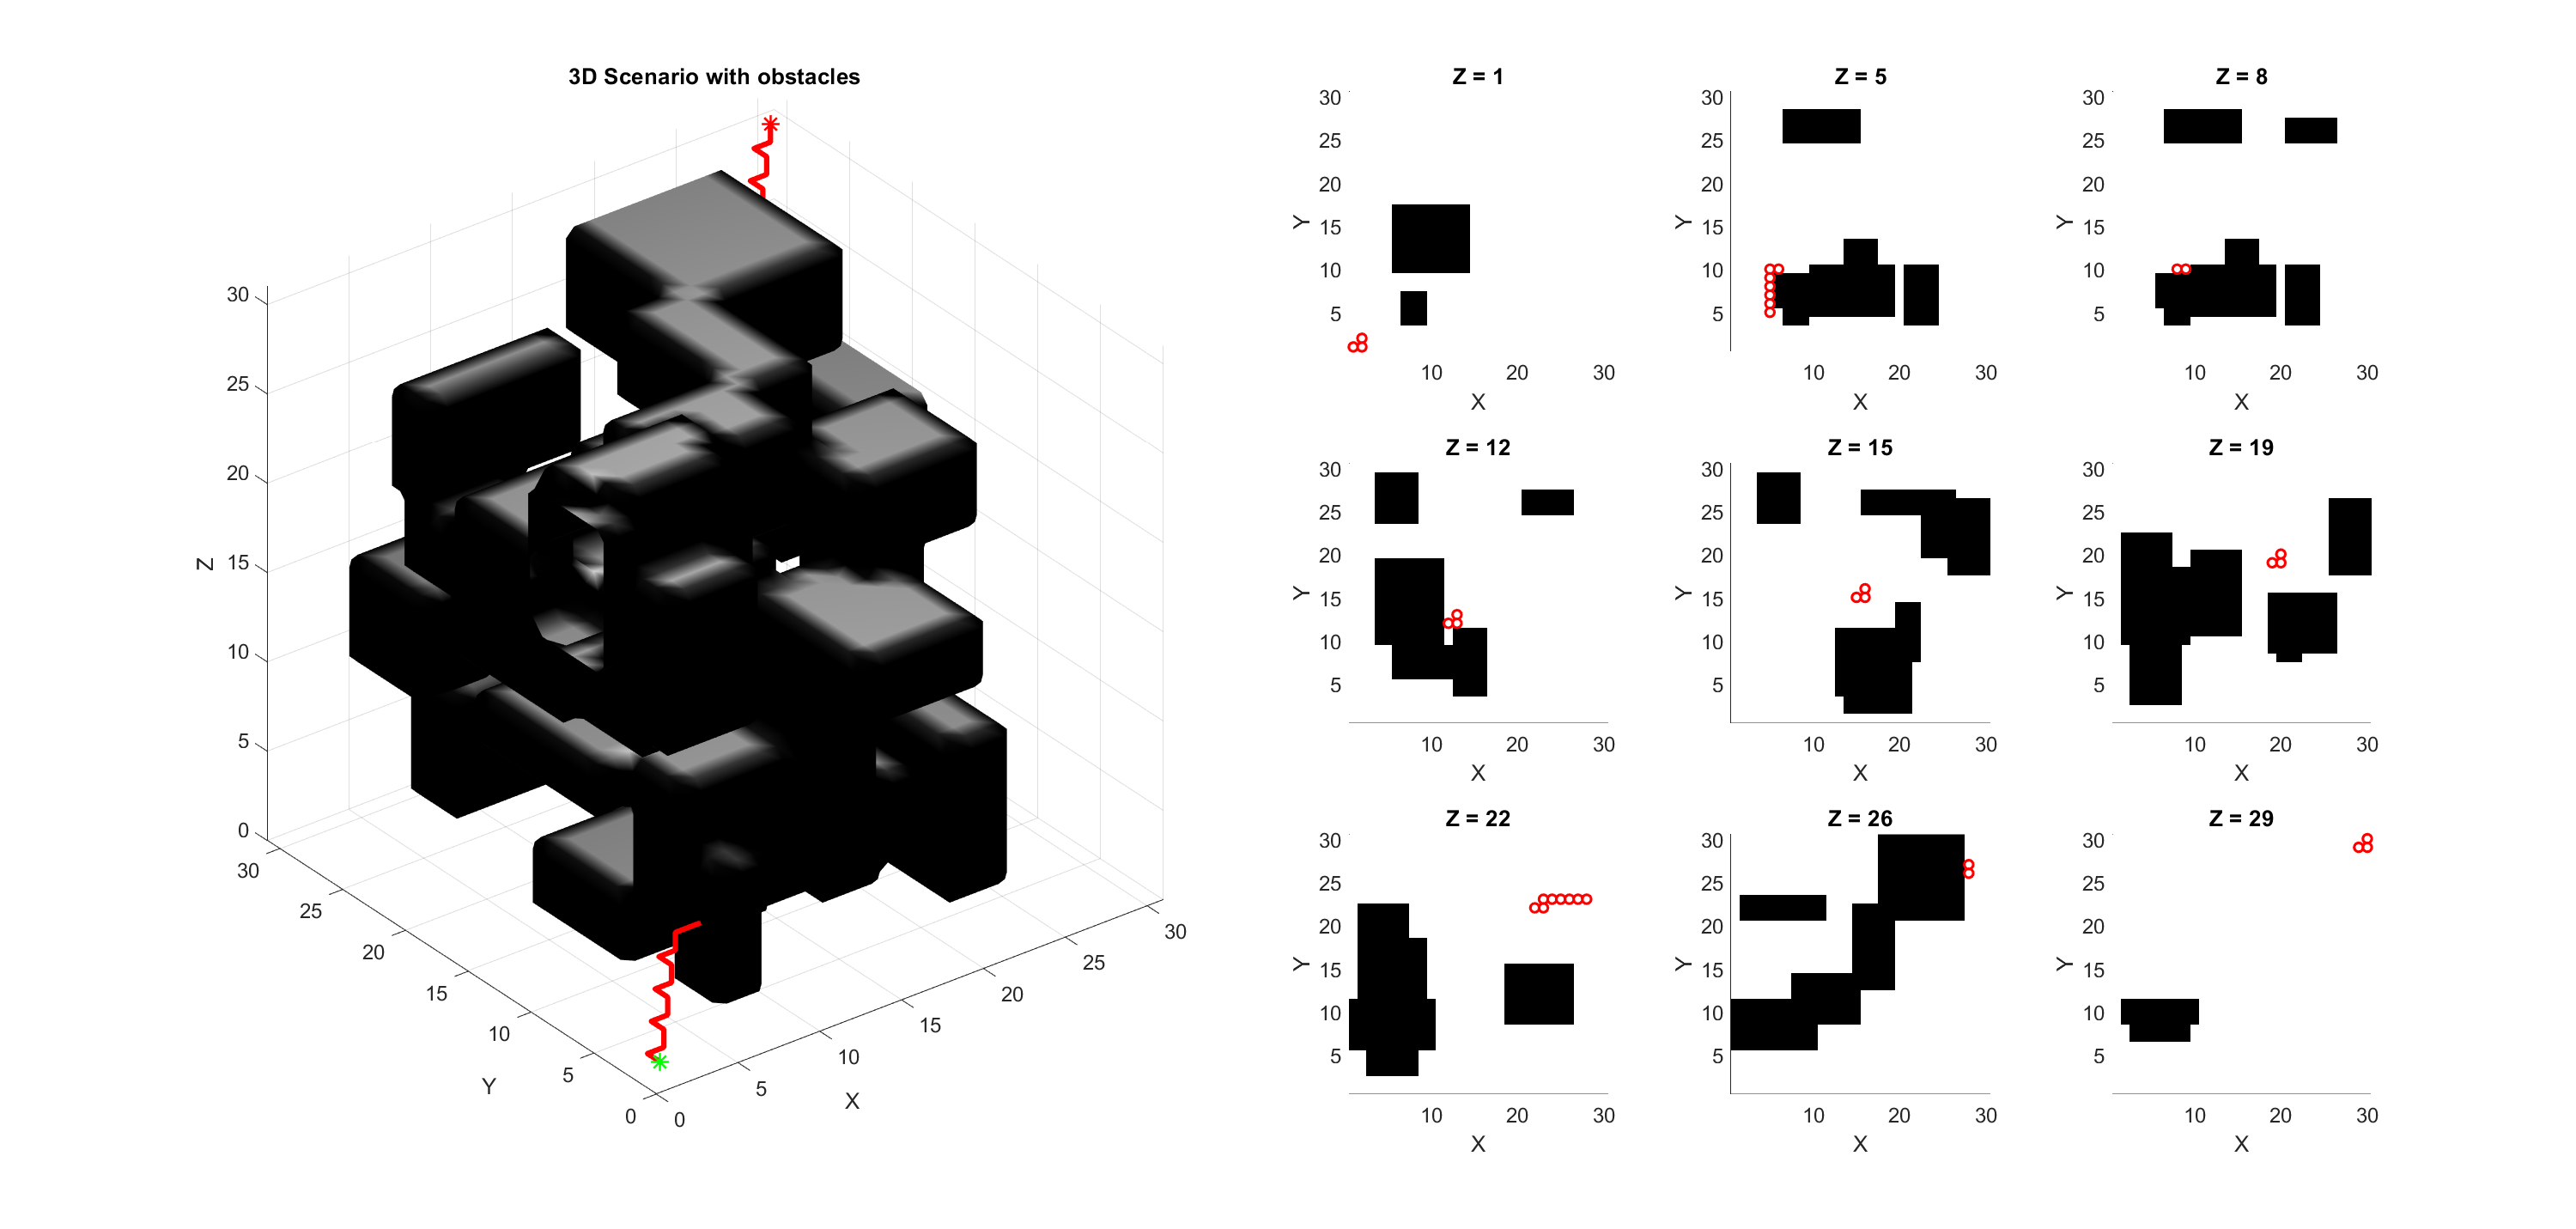
\includegraphics[width=1.0\textwidth]{./img/MATLAB/multidim/3D_a_star.pdf}
    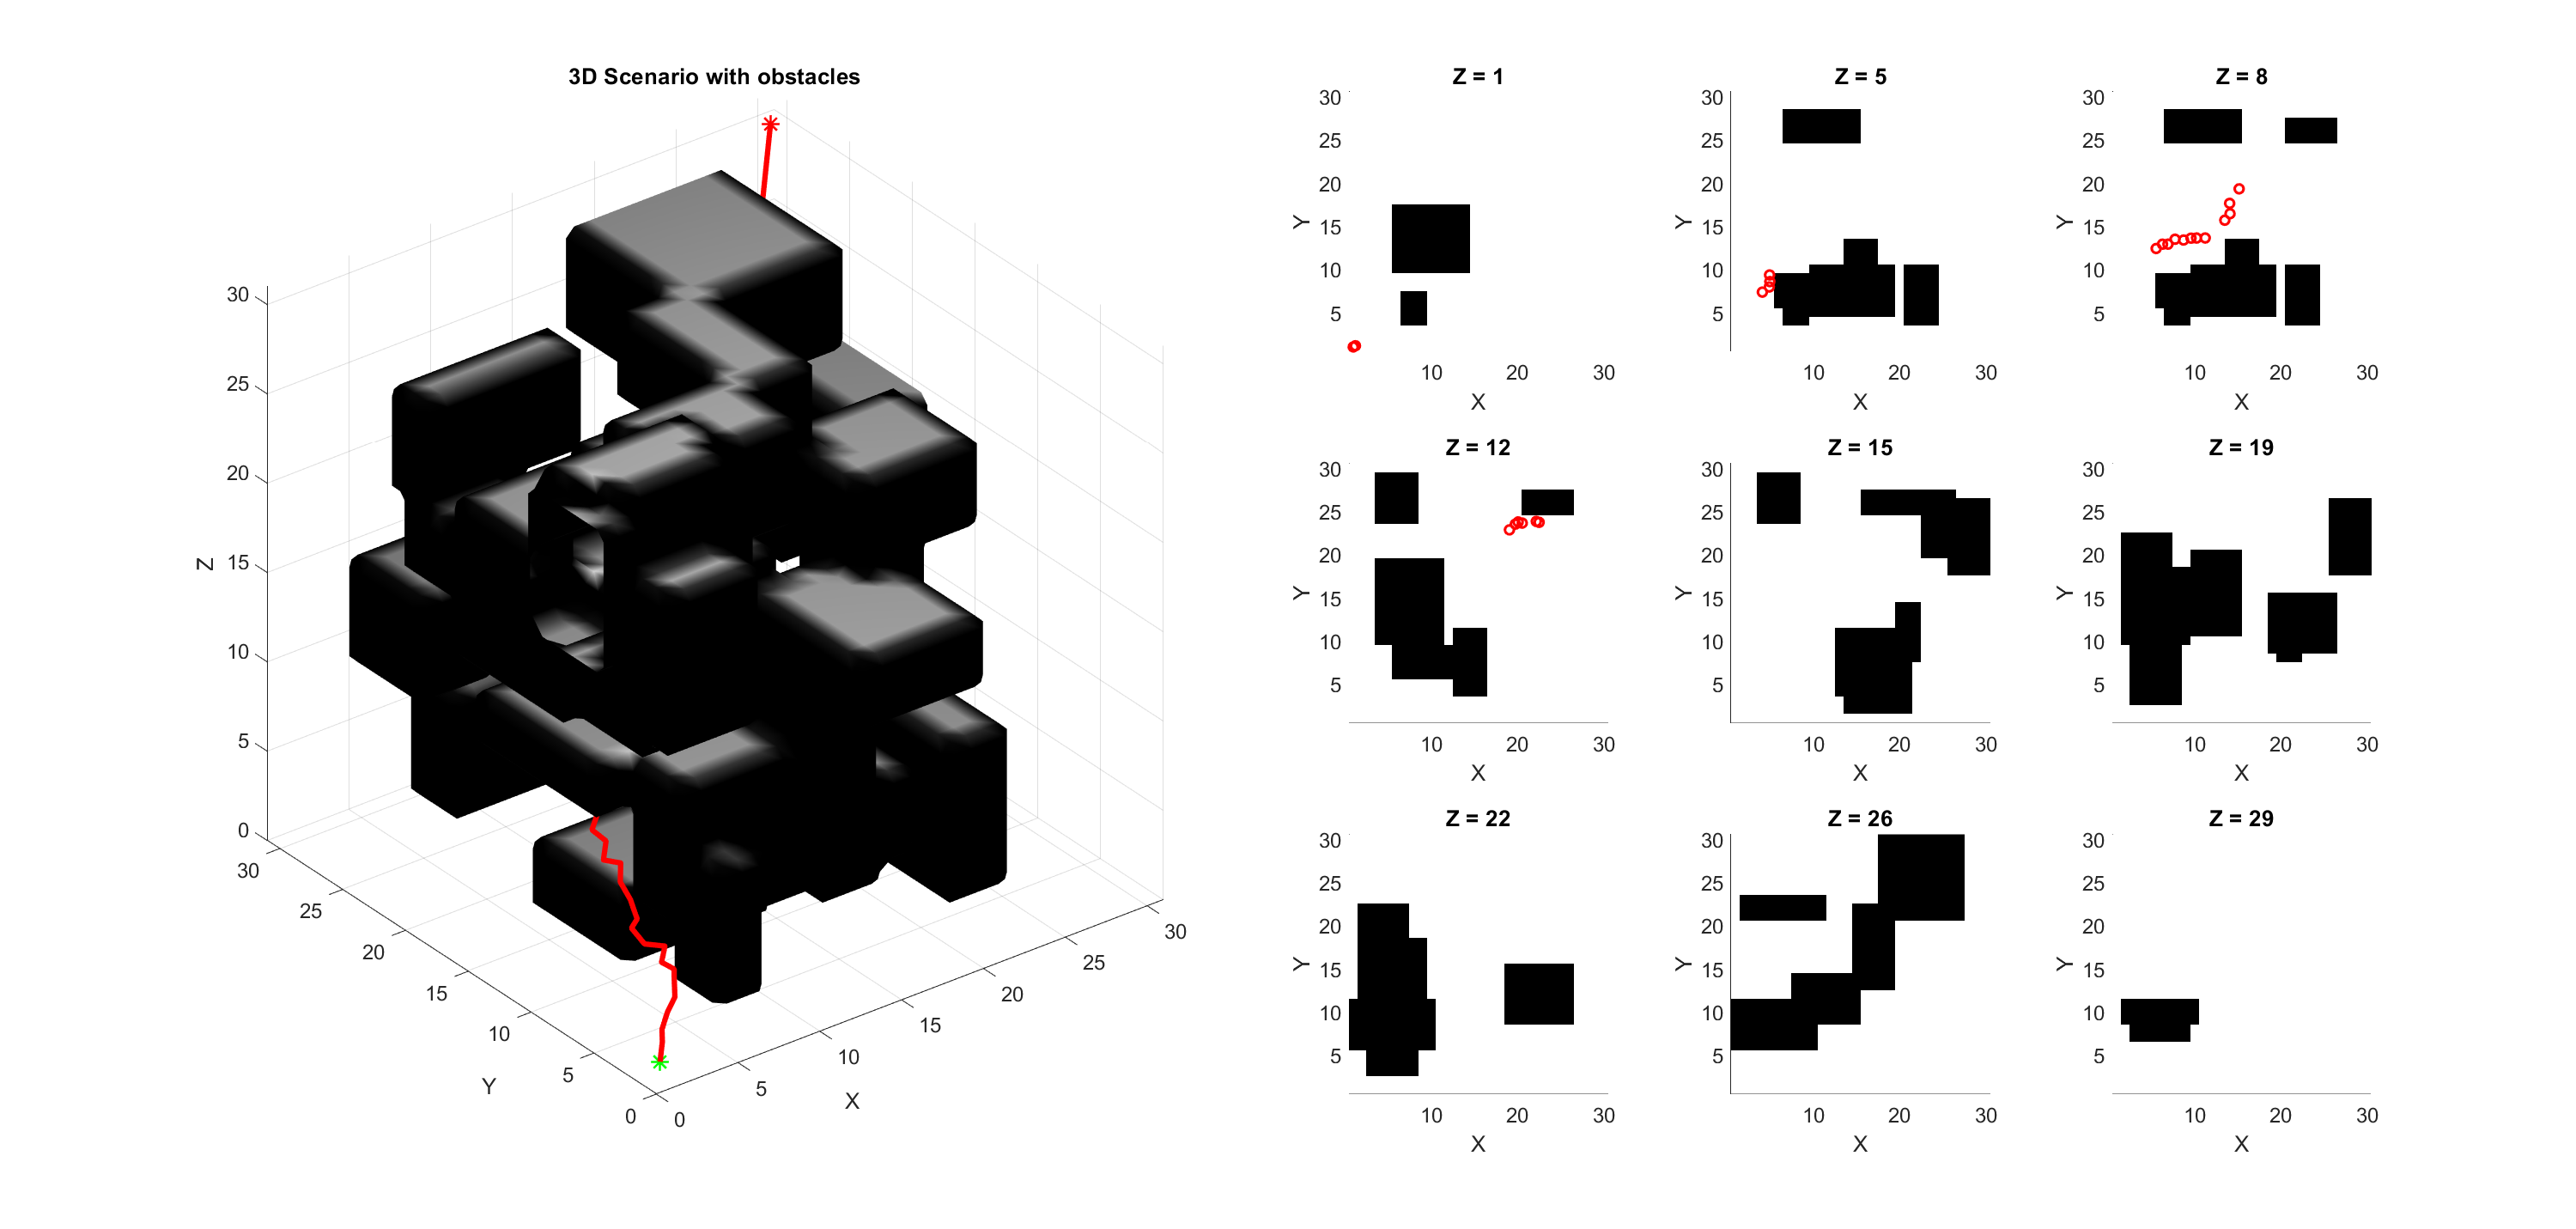
\includegraphics[width=1.0\textwidth]{./img/MATLAB/multidim/3D_rrt.pdf}
    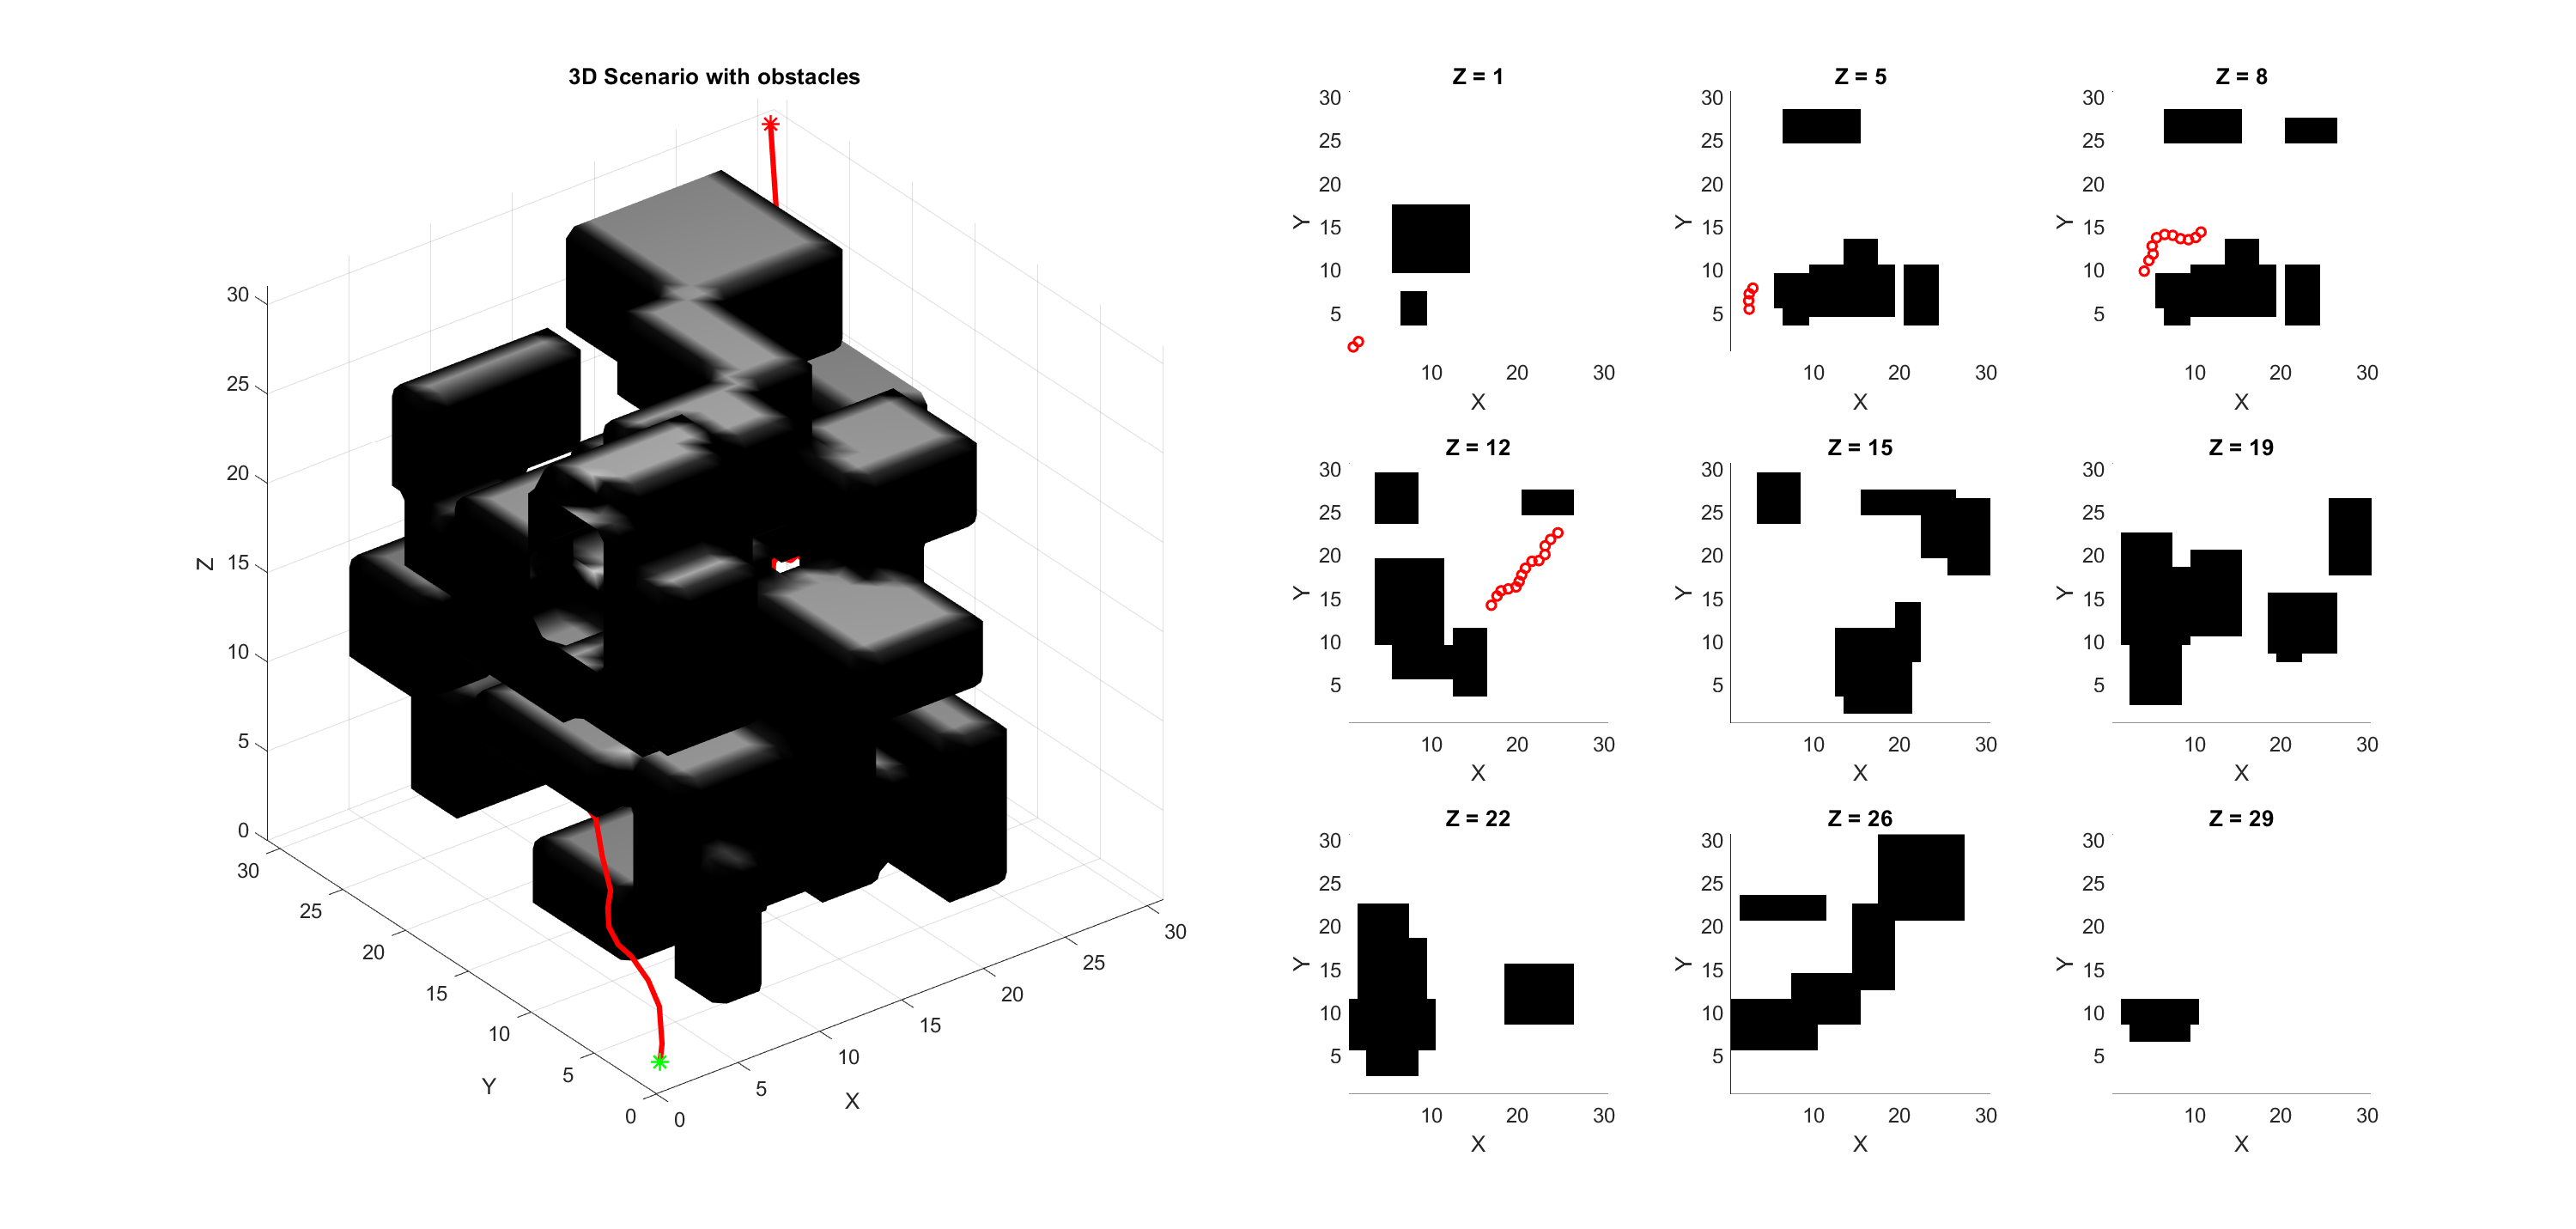
\includegraphics[width=1.0\textwidth]{./img/MATLAB/multidim/3D_rrt_star.pdf}
    \caption{Path generated by A* (top), RRT (middle) and RRT* (bottom) algorithms on the same 3D scenario.}
    \label{fig:3D_grid_vs_sample_based}
\end{figure}

From Table \ref{tab:3D_grid_vs_sample_based} it's clear how the use of grid-based algorithm for single-query planning problem is unfeasible.
These tests, again, highlight the strong adaptability of the sample-based algorithms to high-dimensional problems, while grid-based algorithms are not able to cope with the increased complexity of the problem.

Notice that a minor modification to both the RRT and RRT* algorithms have been applied in order to further reduce the computational time.
In particular, we have found that the original algorithms excelled at fast exploration of the workspace, reaching in little amount of time every distinct volume closed by obstacles.
However, once arrived at the volume of the goal configuration, they failed in creating the final connection and close the planning problem.
In order to avoid useless sampling, we have added a simple logic inside the main algorithm loop that checks if the euclidean connection between the lastly added node and the goal is collision-free or not.
By doing so, the time required for planning drops significantly.

Listing \ref{lst:rrt_speed_up} shows the implementation for this strategy.

\begin{lstlisting}[
    style=Matlab-editor,
    caption={Implementation of the fast goal connection for sampling-based algorithm.},
    label={lst:rrt_speed_up}
]
while (Node.euclideanDistance(q_new, node_final.state) > G.step_length && iter < G.max_iter)
    % ...
    if (G.isValidConnection(q_new, node_final.state, map))
        % We have free space along the connection with the goal
        % Stop sampleing and directly add the goal node to the tree
        break
    end
end
\end{lstlisting}